
\begin{minipage}{0.48\linewidth}

La figure ci-après est la copie d’écran d’un programme réalisé avec le logiciel « Scratch ».
\begin{enumerate}
\item Montrer que si on choisit $2$ comme nombre de départ, alors le programme renvoie $-5$.
\item Que renvoie le programme si on choisit au départ :
\begin{enumerate}
\item le nombre $5$ ?
\item le nombre $-4$?
\end{enumerate}
\item Déterminer  les  nombres qu’il faut choisir au départ pour  que  le  programme renvoie 0.
\end{enumerate}

\end{minipage}
\hfill
\begin{minipage}{0.48\linewidth}
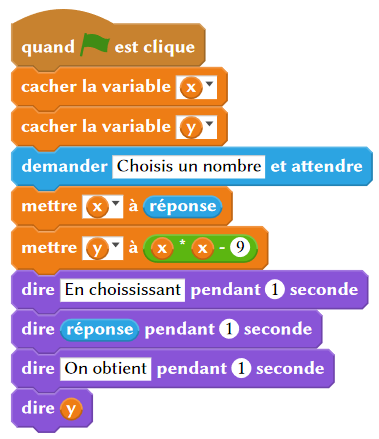
\includegraphics[scale=0.6]{NF-54.png} 
\end{minipage}